%%%%%%%%%%%%%%%%%%%%%%%%%%%%%%%%%%%%%%%%%%%%%%%%%%%
%
%  New template code for TAMU Theses and Dissertations starting Fall 2012.  
%  For more info about this template or the 
%  TAMU LaTeX User's Group, see http://www.howdy.me/.
%
%  Author: Wendy Lynn Turner 
%
%%%%%%%%%%%%%%%%%%%%%%%%%%%%%%%%%%%%%%%%%%%%%%%%%%%

\documentclass[12pt]{report}
\usepackage[letterpaper]{geometry}
\geometry{verbose,tmargin=1.25in,bmargin=1.25in,lmargin=1.4in,rmargin=1.15in}
 \usepackage[doublespacing]{setspace}
 \usepackage{tocloft}
 \usepackage[rm, tiny,center, compact]{titlesec}
 \usepackage{indentfirst}
 \usepackage{etoolbox}
\usepackage{tocvsec2}
 \usepackage[titletoc]{appendix}
 \usepackage{appendix}
 \usepackage{tamuconfig}
\usepackage{rotating}
%Graphics
\usepackage{float}
\usepackage{xcolor,graphicx}
%Math stuff
\usepackage{amsmath}
\usepackage{mathptmx}
\usepackage[mathscr]{euscript}
\newcommand{\vr}{\vec{r}}
\newcommand{\vo}{\vec{\Omega}}
%Changing spacing in itemized lists
\usepackage{enumitem}
\setlist{nosep}
%Include a pdf file
\usepackage{pdfpages}
%Algorithm
\usepackage{algorithm}
\usepackage{algorithmic}
\renewcommand{\arraystretch}{1}
\usepackage{caption}

% Added to fix issues with pdf searching in some versions of LaTeX
%\usepackage[T1]{fontenc}\usepackage{lmodern}
%%%%%%%%%%%%%%%%%%%%%%%%%%%%%

% Hyperref setup below.  You should be able to get away with using uncommenting just the first line.
%\usepackage[hidelinks]{hyperref}

% if \usepackage[hidelinks]{hyperref} doesn't work try this.
% \usepackage{hyperref}  % Hidelinks is an option that removes link visiability.  TAMU Thesis Offices prefers to not see the links. But often doesn't work.  
% 
% \hypersetup{
%     colorlinks=true,
%     linkcolor=black,
%     citecolor=black,
%     filecolor=black,
%     urlcolor=black,
% }
%%%%%%%  End of hyperref setup.  One of these two options should work, but my motto with hyperref is when in doubt, comment it out!
%%%%%%%%%  This hopefully fixes the problem with vertical spacing of section headings at the top of the page..  Commented out in 1.0.7
% \preto\section{%
% \ifnum\value{section}>0\addtocontents{toc}{\vskip-6pt}\fi
% }
% \preto\subsection{%
% \ifnum\value{subsection}=0\addtocontents{toc}{\vskip-6pt}\fi
% \ifnum\value{subsection}>0\addtocontents{toc}{\vskip-6pt}\fi
% } 
%%%%%%%%%%%%%%%%%%%%%%%%%%%%%%%%%%%%%%%%%%%%%%%%%%%%%%

\begin{document}

\renewcommand{\tamumanuscripttitle}{Load Balancing Unstructured Meshes for Massively Parallel Transport Sweeps}
\renewcommand{\tamupapertype}{Thesis}
\renewcommand{\tamufullname}{Tarek Habib Ghaddar}
\renewcommand{\tamudegree}{Master of Science}
\renewcommand{\tamuchairone}{Dr. Jean Ragusa}
% Uncomment out the next line if you have co-chairs.  You will also need to edit the titlepage.tex file.
%\newcommand{\tamuchairtwo}{Additional Chair Name}
\renewcommand{\tamumemberone}{Dr. Jim Morel}
\newcommand{\tamumembertwo}{Dr. Bojan Popov}
\newcommand{\tamumemberthree}{Committee Member3}
\renewcommand{\tamudepthead}{Dr. Yassin Hassan}
\renewcommand{\tamugradmonth}{May}
\renewcommand{\tamugradyear}{2016}
\renewcommand{\tamudepartment}{Nuclear Engineering}


%%%%%%%%%%%%%%%%%%%%%%%%%%%%%%%%%%%%%%%%%%%%%%%%%%%
%
%  New template code for TAMU Theses and Dissertations starting Fall 2012.  
%  For more info about this template or the 
%  TAMU LaTeX User's Group, see http://www.howdy.me/.
%
%  Author: Wendy Lynn Turner 
%	 Version 1.0 
%  Last updated 8/5/2012
%
%%%%%%%%%%%%%%%%%%%%%%%%%%%%%%%%%%%%%%%%%%%%%%%%%%%

%%%%%%%%%%%%%%%%%%%%%%%%%%%%%% 
%% TITLE PAGE
%% The values get updated automatically.  Please do not make changes to this file other than adding/deleting committee members where necessary.
%%%%%%%%%%%%%%%%%%%%%%%%%%%%%%

\providecommand{\tabularnewline}{\\}



\begin{titlepage}
\begin{center}
\MakeUppercase{\tamumanuscripttitle}
\vspace{4em}

A \tamupapertype

by

\MakeUppercase{\tamufullname}

\vspace{4em}

\begin{singlespace}

Submitted to the Office of Graduate and Professional Studies of \\
Texas A\&M University \\

in partial fulfillment of the requirements for the degree of \\
\end{singlespace}

\MakeUppercase{\tamudegree}
\par\end{center}
\vspace{2em}
\begin{singlespace}
\begin{tabular}{ll}
 & \tabularnewline
& \cr
% If you have Co-Chairs comment out the 'Chair of Committee' line below and uncomment the 'Co-Chairs of Committee' line.
Chair of Committee, & \tamuchairone\tabularnewline
%Co-Chairs of Committee, & \tamuchairone\tabularnewline & \tamuchairtwo\tabularnewline
Committee Members, & \tamumemberone\tabularnewline
 & \tamumembertwo\tabularnewline
Head of Department, & \tamudepthead\tabularnewline

\end{tabular}
\end{singlespace}
\vspace{3em}

\begin{center}
\tamugradmonth \hspace{2pt} \tamugradyear

\vspace{3em}

Major Subject: \tamudepartment \par
\vspace{3em}
Copyright \tamugradyear \hspace{.5em}\tamufullname 
\par\end{center}
\end{titlepage}
\pagebreak{}




 % This is simply a file that formats and adds your titlepage, please do not edit this unless you have a specific need. .
%%%%%%%%%%%%%%%%%%%%%%%%%%%%%%%%%%%%%%%%%%%%%%%%%%%
%
%  New template code for TAMU Theses and Dissertations starting Fall 2016.  
%
%
%  Author: Sean Zachary Roberson
%  Version 3.17.09
%  Last Updated: 9/21/2017
%
%%%%%%%%%%%%%%%%%%%%%%%%%%%%%%%%%%%%%%%%%%%%%%%%%%%
%%%%%%%%%%%%%%%%%%%%%%%%%%%%%%%%%%%%%%%%%%%%%%%%%%%%%%%%%%%%%%%%%%%%%
%%                           ABSTRACT 
%%%%%%%%%%%%%%%%%%%%%%%%%%%%%%%%%%%%%%%%%%%%%%%%%%%%%%%%%%%%%%%%%%%%%

\chapter*{ABSTRACT}
\addcontentsline{toc}{chapter}{ABSTRACT} % Needs to be set to part, so the TOC doesnt add 'CHAPTER ' prefix in the TOC.

\pagestyle{plain} % No headers, just page numbers
\pagenumbering{roman} % Roman numerals
\setcounter{page}{2}

\indent The field of radiation transport studies the distribution of radiation throughout a seven-dimensional phase-space consisting of time, space, energy, and direction. Radiation transport is described by the Boltzmann equation and can be solved stochastically or deterministically.

The work presented in this dissertation utilizes the deterministic method known as the transport sweep, a popular technique that has been the subject of a large amount of research.
We specifically focus on the parallel implementations of the transport sweep, and predicting the time it takes to sweep across a structured or unstructured mesh given a set of partitioning parameters, achieved through a time-to-solution estimator, written in Python.
The time-to-solution estimator is tested against PDT, Texas A\&M's massively deterministic transport code.
The time-to-solution estimator's sweep time is within 10\% of PDT's sweep time for the majority of problems tested.

We use the time-to-solution estimator as the objective function in an optimization scheme to attempt to get the partitions that lead to the fastest sweep time for a given problem and partitioning scheme.
Two optimization methods are discussed: using a black box tool (scipy's optimize library) and an intuitive method that relies on placing partitions in mesh locations that does not increase the number of cells (which we chose to name the CDF method).
The time-to-solution estimator proved to not be smooth enough for a black box tool to work, so the geometry based optimization method became the primary method.
The CDF method proved effective for our unbalanced pin test problem, improving the time to solution over previously used partitioning schemes.
For our larger test problem, the optimized partitioning scheme improves the time to solution over one previously used partitioning scheme, but is not as effective relative to other previously used partitioning schemes.
\pagebreak{}

%%%%%%%%%%%%%%%%%%%%%%%%%%%%%%%%%%%%%%%%%%%%%%%%%%%
%
%  New template code for TAMU Theses and Dissertations starting Fall 2016.  
%
%
%  Author: Sean Zachary Roberson
%  Version 3.17.09
%  Last Updated: 9/21/2017
%
%%%%%%%%%%%%%%%%%%%%%%%%%%%%%%%%%%%%%%%%%%%%%%%%%%%


%%%%%%%%%%%%%%%%%%%%%%%%%%%%%%%%%%%%%%%%%%%%%%%%%%%%%%%%%%%%%%%%%%%%%%
%%                           ACKNOWLEDGMENTS
%%%%%%%%%%%%%%%%%%%%%%%%%%%%%%%%%%%%%%%%%%%%%%%%%%%%%%%%%%%%%%%%%%%%%
\chapter*{ACKNOWLEDGMENTS}
\addcontentsline{toc}{chapter}{ACKNOWLEDGMENTS}  % Needs to be set to part, so the TOC doesnt add 'CHAPTER ' prefix in the TOC.


\indent I would like to thank Dr. Jean Ragusa for toeing the line between demanding and understanding perfectly. I know I haven't made your job as my advisor easy. 

Thank you to my committee, Drs. Adams, Amato, and Morel, for the feedback and advice when needed to push this work to completion.

A special thank you to Daryl Hawkins, a man I'm convinced is the most overworked code developer on the planet. This work would have been impossible without him. 

Thank you to Andrew Till for always being a sounding board for academic ideas, and thank you to Ian Halvic for dealing with my less than fine moments in the office. 

Thank you to Dillon Herring for his accelerated effort on his Master's project, which helped the completion of this dissertation.

To Nicolas Quintanar, Brian Ng, and David Saucier, thank you for keeping my life fun and full of life. 

To the CERT team, thank you for your constant support in all of my research endeavors.




\pagebreak{}
%%%%%%%%%%%%%%%%%%%%%%%%%%%%%%%%%%%%%%%%%%%%%%%%%%%
%
%  New template code for TAMU Theses and Dissertations starting Fall 2012.  
%  For more info about this template or the 
%  TAMU LaTeX User's Group, see http://www.howdy.me/.
%
%  Author: Wendy Lynn Turner 
%	 Version 1.0 
%  Last updated 8/5/2012
%
%%%%%%%%%%%%%%%%%%%%%%%%%%%%%%%%%%%%%%%%%%%%%%%%%%%

%%%%%%%%%%%%%%%%%%%%%%%%%%%%%%%%%%%%%%%%%%%%%%%%%%%%%%%%%%%%%%%%%%%%%%
%%                           NOMENCLATURE
%%%%%%%%%%%%%%%%%%%%%%%%%%%%%%%%%%%%%%%%%%%%%%%%%%%%%%%%%%%%%%%%%%%%%

\chapter*{NOMENCLATURE}
\addcontentsline{toc}{chapter}{NOMENCLATURE}  % Needs to be set to part, so the TOC doesnt add 'CHAPTER ' prefix in the TOC.

\begin{tabular}{ll}
B/CS  & Bryan/College Station\tabularnewline
HSUS & Humane Society of the United States\tabularnewline
P & Pressure\tabularnewline
T  & Time\tabularnewline
TVA & Tennessee Valley Authority\tabularnewline
TxDOT \hfill{}\hfill{}\hfill{}\hfill{}\hfill{}\hfill{}\hfill{}\hfill{} & \multicolumn{1}{l}{Texas Department of Transportation}\tabularnewline
\end{tabular}

\vspace{2em}

This page is optional.

\pagebreak{}

%%%%%%%%%%%%%%%%%%%%%%%%%%%%%%%%%%%%%%%%%%%%%%%%%%%
%
%  New template code for TAMU Theses and Dissertations starting Fall 2012.  
%  For more info about this template or the 
%  TAMU LaTeX User's Group, see http://www.howdy.me/.
%
%  Author: Wendy Lynn Turner 
%	 Version 1.7
%  Last updated 3/24/2014
%
%%%%%%%%%%%%%%%%%%%%%%%%%%%%%%%%%%%%%%%%%%%%%%%%%%%
%%%%%%%%%%%%%%%%%%%%%%%%%%%%%%%%%%%%%%%%%%%%%%%%%%%%%%%%%%%%%%%%%%%%%%
%%       TABLE OF CONTENTS
%%%%%%%%%%%%%%%%%%%%%%%%%%%%%%%%%%%%%%%%%%%%%%%%%%%%%%%%%%%%%%%%%%%%%
% single-space sections in Table of Contents  - commented in version 1.7
%\renewcommand{\cftsecafterpnum}{\vskip0.5\baselineskip}
%\renewcommand{\cftsubsecafterpnum}{\vskip0.5\baselineskip}
%\renewcommand{\cftsubsubsecafterpnum}{\vskip0.5\baselineskip}
%%%%%%%%%%%%%%%%%%%%%%%%%%%%%%%%%%%%%%%%%%%%%%%%%%%

\phantomsection
\addcontentsline{toc}{chapter}{TABLE OF CONTENTS}  

\begin{singlespace}
\renewcommand\contentsname{\normalfont} {\centerline{TABLE OF CONTENTS}}

%\setcounter{tocdepth}{4} % This puts \subsubsection[]{×} in your List of Tables.  The default is 3.


%%%%%%%%%%%%%  Adds Page above the page number in TOC
\setlength{\cftaftertoctitleskip}{1em}
\renewcommand{\cftaftertoctitle}{%
\hfill{\normalfont {Page}\par}}



\tableofcontents

\end{singlespace}

\pagebreak{}

%%%%%%%%%%%%%%%%%%%%%%%%%%%%%%%%%%%%%%%%%%%%%%%%%%%%%%%%%%%%%%%%%%%%%%
%%                           LIST OF FIGURES
%%%%%%%%%%%%%%%%%%%%%%%%%%%%%%%%%%%%%%%%%%%%%%%%%%%%%%%%%%%%%%%%%%%%%

\phantomsection
\addcontentsline{toc}{chapter}{LIST OF FIGURES}  

\renewcommand{\cftloftitlefont}{\center\normalfont\MakeUppercase}

\setlength{\cftbeforeloftitleskip}{-12pt} %% Positions the LOF title vertically to match the chapter titles
\renewcommand{\cftafterloftitleskip}{12pt}


\renewcommand{\cftafterloftitle}{%
\\[4em]\mbox{}\hspace{2pt}FIGURE\hfill{\normalfont Page}\vskip\baselineskip}

\begingroup


\begin{center}
\begin{singlespace}
%% These values make the lof table entries appear double spaced between.
\setlength{\cftbeforechapskip}{0.4cm}
\setlength{\cftbeforesecskip}{0.30cm}
\setlength{\cftbeforesubsecskip}{0.30cm}
\setlength{\cftbeforefigskip}{0.4cm}
\setlength{\cftbeforetabskip}{0.4cm} 

\listoffigures

\end{singlespace}
\end{center}

\pagebreak{}


%%%%%%%%%%%%%%%%%%%%%%%%%%%%%%%%%%%%%%%%%%%%%%%%%%%%%%%%%%%%%%%%%%%%%%
%%                           lIST OF TABLES
%%%%%%%%%%%%%%%%%%%%%%%%%%%%%%%%%%%%%%%%%%%%%%%%%%%%%%%%%%%%%%%%%%%%%%
%
\phantomsection
\addcontentsline{toc}{chapter}{LIST OF TABLES}  

\renewcommand{\cftlottitlefont}{\center\normalfont\MakeUppercase}

\setlength{\cftbeforelottitleskip}{-12pt} %% Positions the LOT title vertically to match the chapter titles

\renewcommand{\cftafterlottitleskip}{12pt}


\renewcommand{\cftafterlottitle}{%
\\[4em]\mbox{}\hspace{4pt}TABLE\hfill{\normalfont Page}\vskip\baselineskip}

\begin{center}
\begin{singlespace}

%% These values make the lot table entries appear double spaced between.
\setlength{\cftbeforechapskip}{0.4cm}
\setlength{\cftbeforesecskip}{0.30cm}
\setlength{\cftbeforesubsecskip}{0.30cm}
\setlength{\cftbeforefigskip}{0.4cm}
\setlength{\cftbeforetabskip}{0.4cm}

\listoftables 

\end{singlespace}
\end{center}
\endgroup
\pagebreak{}  % Need this for the pagenumbering to be correct.   % This is simply a file that formats and adds your toc, lof, and lot, please do not edit this unless you have a specific need. .

%%%%%%%%%%%%%%%%%%%%%%%%%%%%%%%%%%%%%%%%%%%%%%%%%%%
%
%  New template code for TAMU Theses and Dissertations starting Fall 2016.
%
%
%  Author: Sean Zachary Roberson
%  Version 3.17.09
%  Last Updated: 9/21/2017
%
%%%%%%%%%%%%%%%%%%%%%%%%%%%%%%%%%%%%%%%%%%%%%%%%%%%

%%%%%%%%%%%%%%%%%%%%%%%%%%%%%%%%%%%%%%%%%%%%%%%%%%%%%%%%%%%%%%%%%%%%%%
%%                           Introduction
%%%%%%%%%%%%%%%%%%%%%%%%%%%%%%%%%%%%%%%%%%%%%%%%%%%%%%%%%%%%%%%%%%%%%


\pagestyle{plain} % No headers, just page numbers
\pagenumbering{arabic} % Arabic numerals
\setcounter{page}{1}


\chapter{\uppercase {INTRODUCTION}}\label{cha:introduction}

The field of radiation transport studies the behavior of radiation throughout a six-dimensional phase space of time, space, energy, and direction. 
Radiation transport is commonly used for radiation shielding and criticality safety applications, as well as the general simulation of radiation in different environments. 

Radiation transport can be solved stochasticly or deterministicly.
The Monte Carlo method is used for stochastic radiation transport by tracking the behavior of a finite number of particles from their ``birth'' (for example, a neutron source) until their ``death'' (getting absorbed or escaping through a problem boundary), and statistically evaluating relevant quantities of interest (for example, neutron flux in a detector) \cite{shultis_mc}.
Codes such as MCNP \cite{MCNP} and SHIFT {\cite{shift} utilize the Monte Carlo method to perform high fidelity radiation transport simulations for a variety of experiments and problems. 

Deterministic transport discretizes the time, spatial, energy, and angular variables to obtain a numerical solution to the transport equation.
There are multiple popular methods to do this such as the method of characteristics and the transport sweeps, implemented by codes such as MPACT \cite{mpact}, Partisn \cite{partisn}, Denovo \cite{denovo}, and PDT \cite{mpadams2013,mpadams2015}. 

The work presented in this dissertation utilizes the transport sweep, a method that discretizes the Boltzmann transport equation \cite{bell_glasstone,zweifel,davison,duderstadt} down to a system of algebraic equations that can then be solved iteratively \cite{adams_larsen}.
It is often desirable to split the full system so that the memory cost can be distributed across multiple processors. 
The smaller linear system matrices often exhibit a lower block triangular structure whose solutions are easy to obtain.
With each block being thought of as a cell, the solution is obtained by following the flow of radiation, or ``marching'' through a mesh.

This ``marching'' or ``sweeping'' through a mesh gains complexity for unstructured and/or distributed meshes. Partitioning meshes in a balanced (or near equivalent amount of work per processor) fashion that preserves mesh integrity can present challenges.
In addition, maintaining sweep performance for massively parallel simulations has and continues to be a thriving research topic.
The following dissertation chapters will discuss a brief history of the transport sweep, parallel transport sweeps, load balancing unstructured meshes for transport, a time-to-solution estimator, and optimizing partitions for parallel transport. 

\section{The Deterministic Transport Sweep}

Chapter \ref{cha:transport_sweeps} introduces the steady-state neutron transport equation and the discretization process to obtain the discrete form of the transport equation. Chapter \ref{cha:transport_sweeps} also provides more details on the transport sweep.

\section{Parallel Transport Sweeps}

Massively parallel transport sweeps have been shown to scale up to 1.5 million cores on logically Cartesian grids using Texas A\&M's flagship deterministic transport code, PDT \cite{mpadams2013,mpadams2015}.
Chapter \ref{cha:parallel_transport} describes the basics of a parallel sweep algorithm, and specifically describes the KBA algorithm \cite{KBA} and PDT's extension of the KBA algorithm.
This chapter also describes PDT's performance model, which predicts the sweep time given a set of partitioning parameters.

\section{Unstructured Meshing and Load Balancing in PDT}

In order to solve a wider set of problems, an unstructured meshing capability was implemented in PDT.
However, unstructured meshes may lead to imbalanced partitions, or different numbers of mesh cells per processor.
To address this, two load-balancing algorithms have been implemented in PDT, the original load-balancing algorithm and the load-balancing-by-dimension algorithm \cite{mastersthesis,mc2017}.

\section{Time-to-Solution Estimator}

PDT's existing performance model does not account for unstructured meshes and imbalanced partitions.
Chapter \ref{cha:tts} describes the time-to-solution estimator, a graph-based method that estimates the time it takes to sweep across a problem given a mesh, partitioning scheme, and machine-specific parameters.

\section{Partitioning Optimization}

The time-to-solution estimator described in Chapter \ref{cha:tts} is used to optimize the partitioning scheme.
Chapter \ref{cha:optimization} details two optimization methods: a ``black box'' method that uses Python's scipy.optimize library and a ``human-intelligence'' method that prioritizes partition placement in locations that don't add cells to a mesh.

%\pagestyle{plain} % No headers, just page numbers
%\pagenumbering{arabic} % Arabic numerals
%\setcounter{page}{3}

\chapter{\uppercase {The Transport Equation}}
\label{ch:transporteq} 

The steady-state neutron transport equation describes the behavior of neutrons in a medium and is given by Eq.~\eqref{continuous transport}:
\begin{multline}
\vo \cdot \vec \nabla \psi(\vr,E,\vo) +\Sigma_t(\vr,E) \psi(\vr,E,\vo)  = \\
\int_{0}^{\infty}dE' \int_{4\pi}d\Omega' \Sigma_s(\vr,E'\to E, \Omega'\to\Omega)\psi(\vr,E',\vo') 
+ S_{ext}(\vr,E,\vo) ,
\label{continuous transport}
\end{multline}
where $\vec{\Omega}\cdot \vec\nabla\psi$ is the leakage term and $\Sigma_t\psi$ is the total collision term (absorption, outscatter, and within group scattering). These are the loss terms of the neutron transport equation. The right hand side of Eq.~\eqref{continuous transport} represents the gain terms, where $S_{ext}$ is the external source of neutrons and $\int_{0}^{\infty}dE'\int_{4\pi}d\Omega'\Sigma_s(E'\to E, \Omega'\to\Omega)\psi(\vr,E',\vo')$ is the inscatter term, which represents all neutrons scattering from energy $E'$ and direction $\vo'$ into energies about $E$ and directions about $\vo$. 

Without loss of generality for the research problem at hand, we assume isotropic scattering for simplicity. The double differential scattering cross section, $\Sigma_s(E'\to E, \Omega'\to\Omega)$, no longer depends on direction and is divided by $4\pi$ to reflect isotropic behavior. This yields:
\begin{multline}
\label{isotropic}
\vo \cdot \vec \nabla \psi(\vr,E,\vo) +\Sigma_t(\vr,E) \psi(\vr,E,\vo) \\ = \frac{1}{4\pi}\int_{0}^{\infty}dE' \Sigma_s(\vr,E'\to E) \int_{4\pi}d\Omega' \psi(\vr,E',\vo')  + S_{ext}(\vr,E,\vo) \nonumber
\end{multline}
\begin{equation}
\vo \cdot \vec \nabla \psi(\vr,E,\vo) +\Sigma_t(\vr,E) \psi(\vr,E,\vo) = \frac{1}{4\pi}\int_{0}^{\infty}dE' \Sigma_s(\vr,E'\to E) \phi(\vr,E')  + S_{ext}(\vr,E,\vo) ,
\end{equation}
where we have introduced the scalar flux as the integral of the angular flux:
\begin{equation}
\label{def_scalar_flux}
\phi(\vr,E') = \int_{4\pi}d\Omega' \psi(\vr,E',\vo').
\end{equation}
The next step to solving the transport equation is to discretize in energy, yielding Eq.~\eqref{multigroup} the multigroup transport equation:
\begin{equation}
\vo \cdot \vec \nabla \psi_g(\vr,\vo) +\Sigma_{t,g}(\vr) \psi_g(\vr,\vo) = \frac{1}{4\pi}\sum_{g^{\prime}}\Sigma_{s,g^{\prime}\to g}(\vr)\phi_{g^{\prime}}(\vr) + S_{ext,g}(\vr,\vo), \quad \text{for } 1 \le g \le G
\label{multigroup}
\end{equation}
where the multigroup transport equations now form a system of coupled equations. 

Next, we discretize in angle using the discrete ordinates method, whereby an angular quadrature $\left( \vo_m, w_m \right)_{1 \le m \le M}$ is used to solve the above equations along a given set of directions $\vo_m$:
\begin{equation}
\vo_m \cdot \vec \nabla \psi_{g,m}(\vr) +\Sigma_{t,g}(\vr) \psi_{g,m}(\vr)  = \frac{1}{4\pi}\sum_{g^{\prime}}\Sigma_{s,g^{\prime}\to g}(\vr)\phi_{g^{\prime}}(\vr) + S_{ext,g,m}(\vr),
\label{angle}
\end{equation}
where the subscript $m$ is introduced to describe the angular flux in direction $m$. We notice that the subscript is not added to our inscatter term because of the isotropic scattering assumption and because the scalar flux does not depend on angle. However, in order to evaluate the scalar flux, we employ the angular weights $w_m$ and the angular flux solutions
$\psi_m$ to numerically perform the angular integration:
\begin{equation}
\label{def_scalar_flux_2}
\phi_g(\vr) \approx \sum_{m=1}^{m=M} w_m \psi_{g,m}(\vr).
\end{equation}

From Equation~\eqref{multigroup}, it is clear that we are solving a sequence of transport equations, one equation per group. Therefore, all transport equations are of the following form:
\begin{equation}
\vo_m \cdot \vec \nabla \psi_{m}(\vr) +\Sigma_{t}(\vr) \psi_{m}(\vr)  = \frac{1}{4\pi}\Sigma_{s}(\vr)\phi(\vr) + q^{ext+inscat}_m(\vr) = q_m(\vr),
\end{equation}
where the group index notation is omitted for brevity.

In order to obtain the solution for this discrete form of the transport equation, an iterative process called source iteration is introduced. This is shown below for the one-group transport equation, Eq. ~\eqref{iteration}:
\begin{equation}
\vo_m \cdot \vec\nabla \psi_m^{(l+1)}(\vr) + \Sigma_t \psi_m^{(l+1)}(\vr) = q_m^{(l)}(\vr),
\label{iteration}
\end{equation}
where the right hand side terms of Eq.~\eqref{angle} have been combined into one general source term, $q_m$. The angular flux of iteration $(l+1)$ is calculated using the $(l^{th})$ value of the scalar flux.

After the angular and energy dependence have been accounted for, Eq.~\eqref{iteration} must be discretized in space as well. We use a discontinuous Galerkin approximation in space,  and the solution across a cell interface is connected based on an upwind approach, where face outflow radiation becomes face inflow radiation for the downwind cells. The solution is obtained by meshing the domain and solving the spatial problem one cell at a time for a given direction. Sweeping the mesh and solving one cell at a time is possible utilizing one of three popular discretization techniques: finite difference\cite{fd}, finite volume\cite{fd}, or discontinuous finite element\cite{Reed}. Figure \ref{sweeps} shows the sweep ordering for a given direction on both a structured and unstructured mesh.

\noindent\begin{minipage}{\textwidth}
\centering
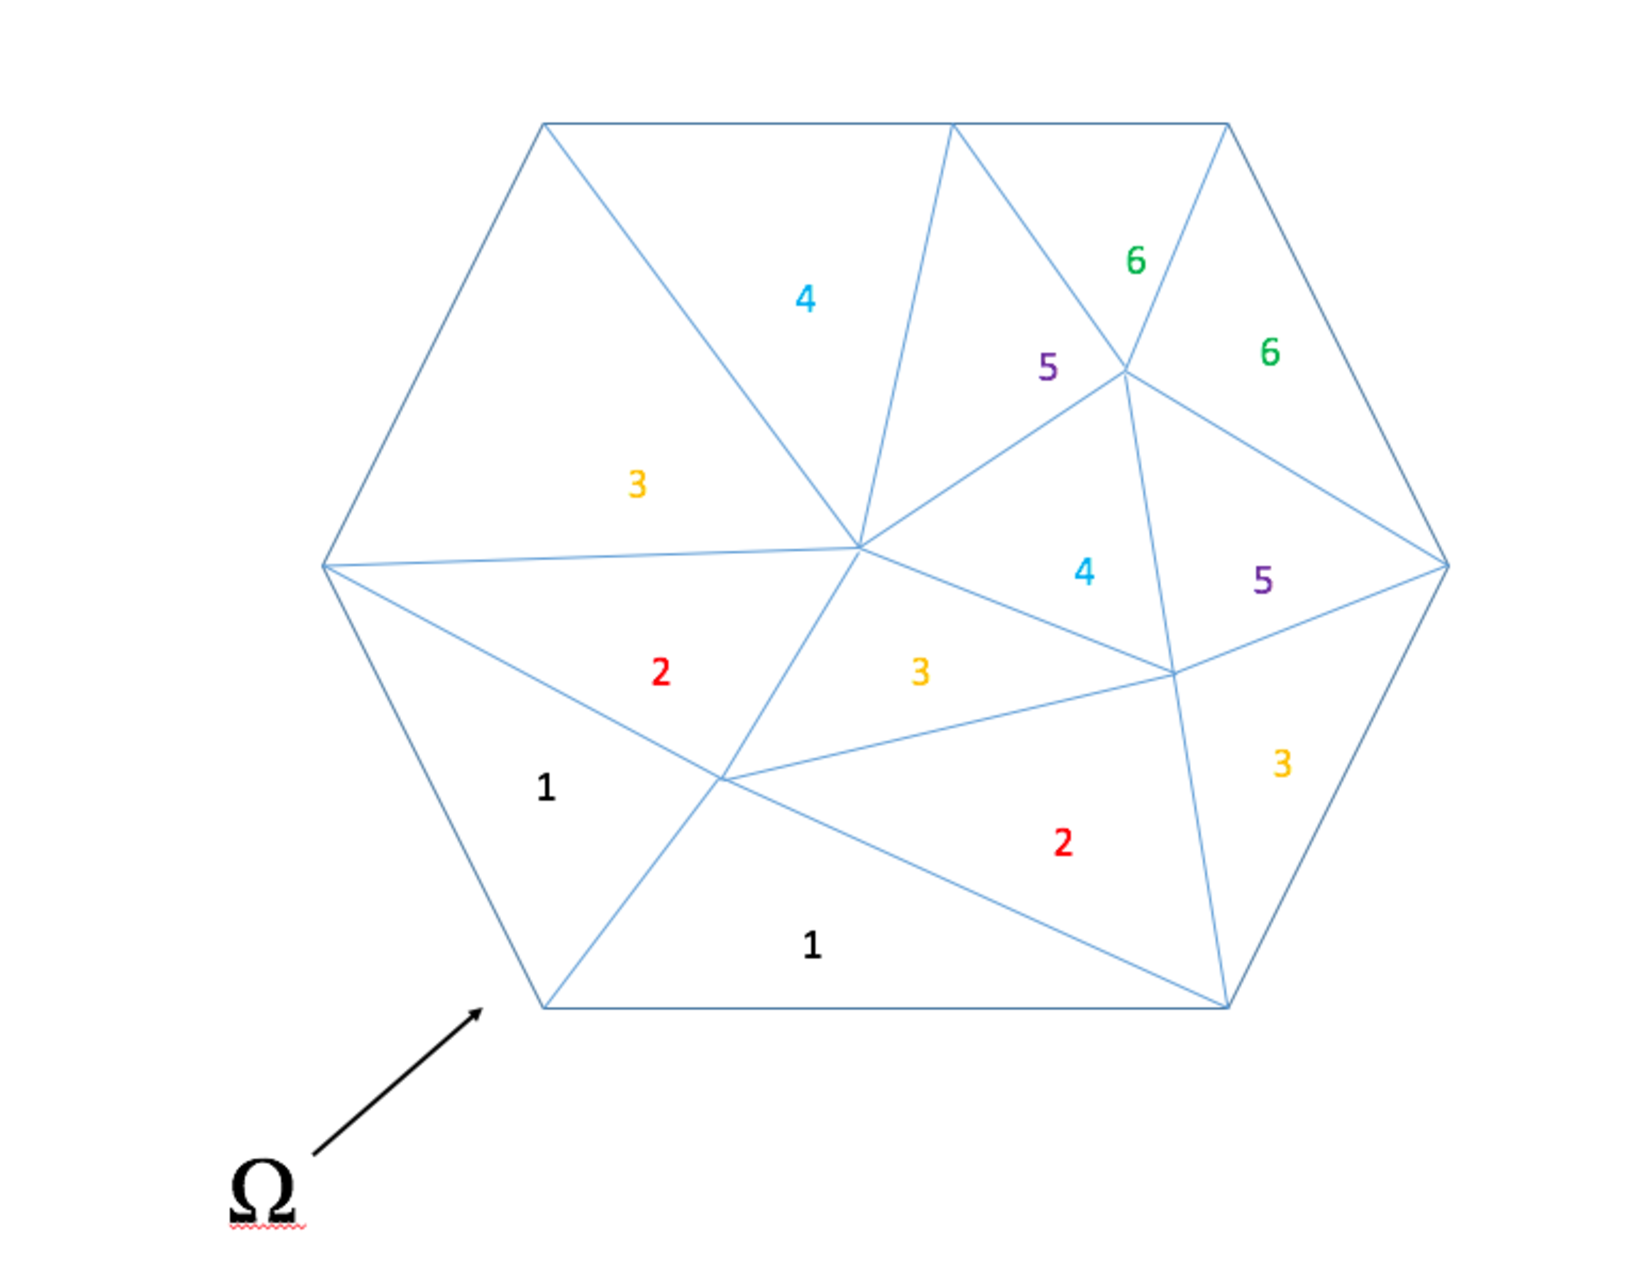
\includegraphics[scale = 0.27]{figures/UnstructureMesh.pdf}
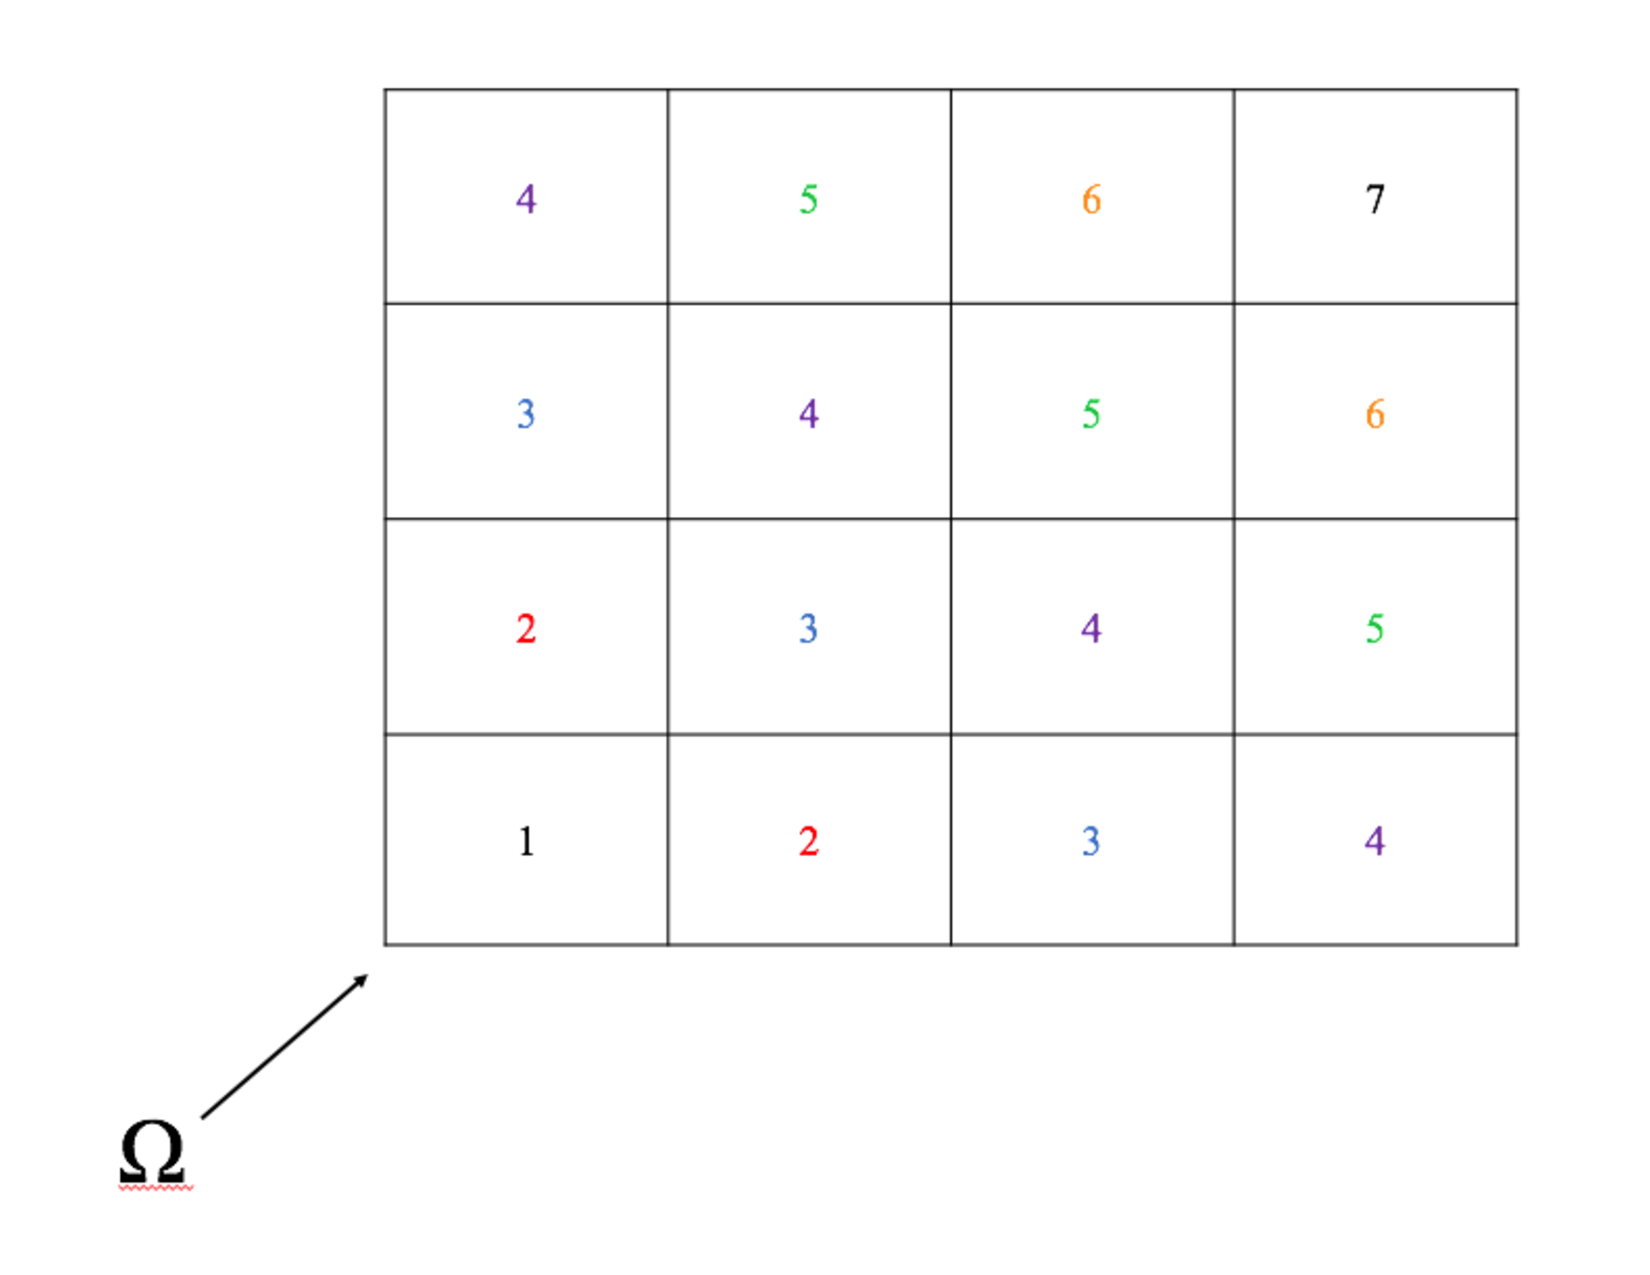
\includegraphics[scale = 0.27]{figures/StructuredMesh.pdf}
\captionof{figure}{A demonstration of a sweep on a structured and unstructured mesh. }
\label{sweeps}
\end{minipage}
\smallskip

The number in each cell represents the order in which the cells are solved. All cells must receive the solution downwind from them before solving for their own solution. This dependency can be represented and stored as a task dependence graph, shown in Fig. \ref{tdg}.

\noindent\begin{minipage}{\textwidth}
\centering
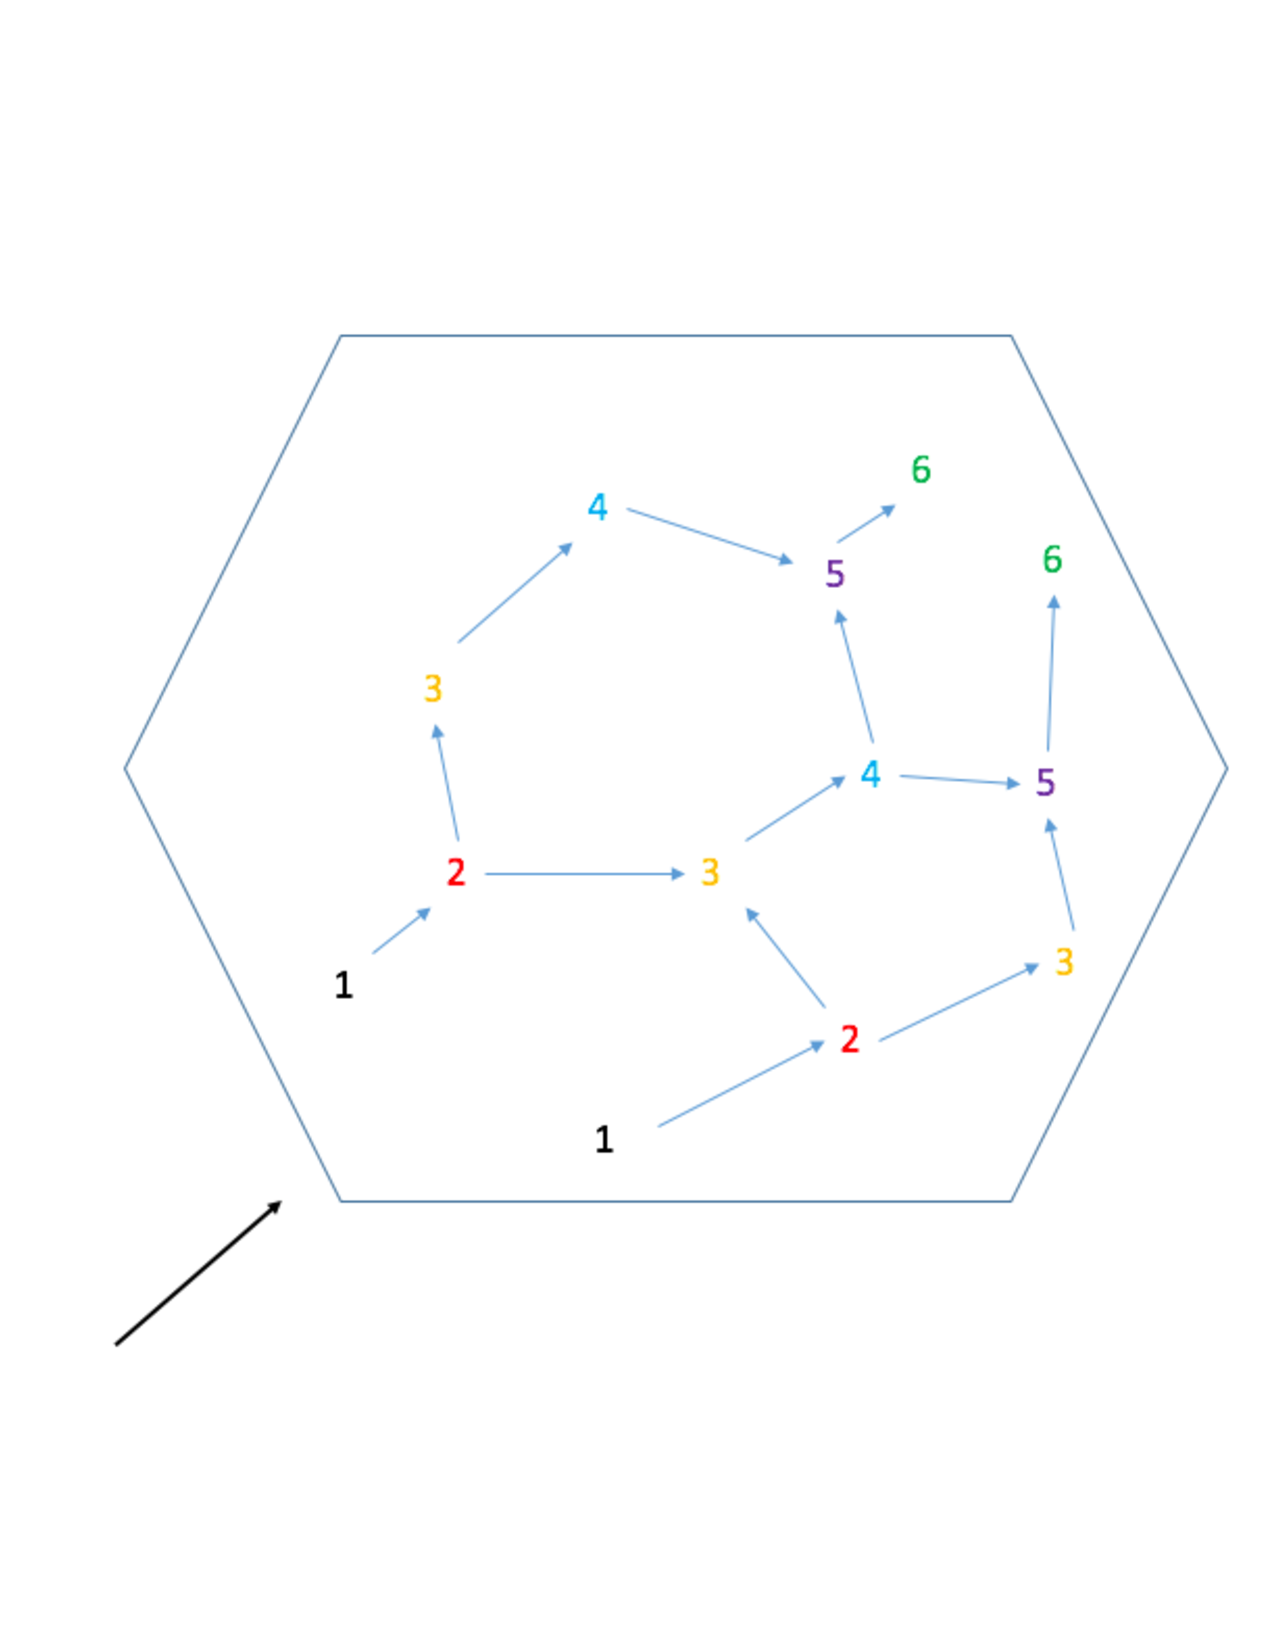
\includegraphics[scale = 0.5,trim = 0cm 3.5cm 0cm 3cm,clip]{figures/tdg.pdf}
\captionof{figure}{A task dependence graph of the unstructured mesh example in Fig. \ref{sweeps}.}
\label{tdg}
\end{minipage}
\smallskip


fix spacing in bibliography, if any...
%%%%%%%%%%%%%%%%%%%%%%%%%%%%%%%%%%%%%%%%%%%%%%%%%%%%%%%%%%%%%
\let\oldbibitem\bibitem
\renewcommand{\bibitem}{\setlength{\itemsep}{0pt}\oldbibitem}
%%%%%%%%%%%%%%%%%%%%%%%%%%%%%%%%%%%%%%%%%%%%%%%%%%%%%%%%%%%%%%%
%%%%%%%%%%%%%%%%%%%%%%%%%%%%%%%%%%%%%%%%%%%%%%%%%%%
%
%  New template code for TAMU Theses and Dissertations starting Fall 2012.  
%  For more info about this template or the 
%  TAMU LaTeX User's Group, see http://www.howdy.me/.
%
%  Author: Wendy Lynn Turner 
%	 Version 1.0 
%  Last updated 8/5/2012
%
%%%%%%%%%%%%%%%%%%%%%%%%%%%%%%%%%%%%%%%%%%%%%%%%%%%


%%%%%%%%%%%%%%%%%%%%%%%%%%%%%%%%%%%%%%%%%%%%%%%%%%%%%%%%%%%%%%%%%%%%%%
%%                           REFERENCES 
%%%%%%%%%%%%%%%%%%%%%%%%%%%%%%%%%%%%%%%%%%%%%%%%%%%%%%%%%%%%%%%%%%%%%

\phantomsection
\addcontentsline{toc}{chapter}{REFERENCES}

\renewcommand{\bibname}{{\normalsize\rm REFERENCES}}

\bibliographystyle{plain}
\bibliography{references}
% %%%%%%%%%%%%%%%%%%%%%%%%%%%%%%%%%%%%%%%%%%%%%%%%%%%
%
%  New template code for TAMU Theses and Dissertations starting Fall 2012.  
%  For more info about this template or the 
%  TAMU LaTeX User's Group, see http://www.howdy.me/.
%
%  Author: Wendy Lynn Turner 
%	 Version 1.0 
%  Last updated 8/5/2012
%
%%%%%%%%%%%%%%%%%%%%%%%%%%%%%%%%%%%%%%%%%%%%%%%%%%%

\begin{appendices}
\titleformat{\chapter}{\centering\normalsize}{APPENDIX \thechapter}{0em}{\vskip .5\baselineskip\centering}
\renewcommand{\appendixname}{APPENDIX}

%%%%%%%%%%%%%%%%%%%%%%%%%%%%%%%%%%%%%%%%%%%%%%%%%%%
%
%  New template code for TAMU Theses and Dissertations starting Fall 2016.
%
%
%  Author: Sean Zachary Roberson 
%	 Version 3.16.09
%  Last updated 9/12/2016
%
%%%%%%%%%%%%%%%%%%%%%%%%%%%%%%%%%%%%%%%%%%%%%%%%%%%

%%%%%%%%%%%%%%%%%%%%%%%%%%%%%%%%%%%%%%%%%%%%%%%%%%%%%%%%%%%%%%%%%%%%%%
%%                           APPENDIX A 
%%%%%%%%%%%%%%%%%%%%%%%%%%%%%%%%%%%%%%%%%%%%%%%%%%%%%%%%%%%%%%%%%%%%%

\phantomsection

\chapter{\uppercase{First Appendix}}

Text for the Appendix follows.

\begin{figure}[H]
\centering
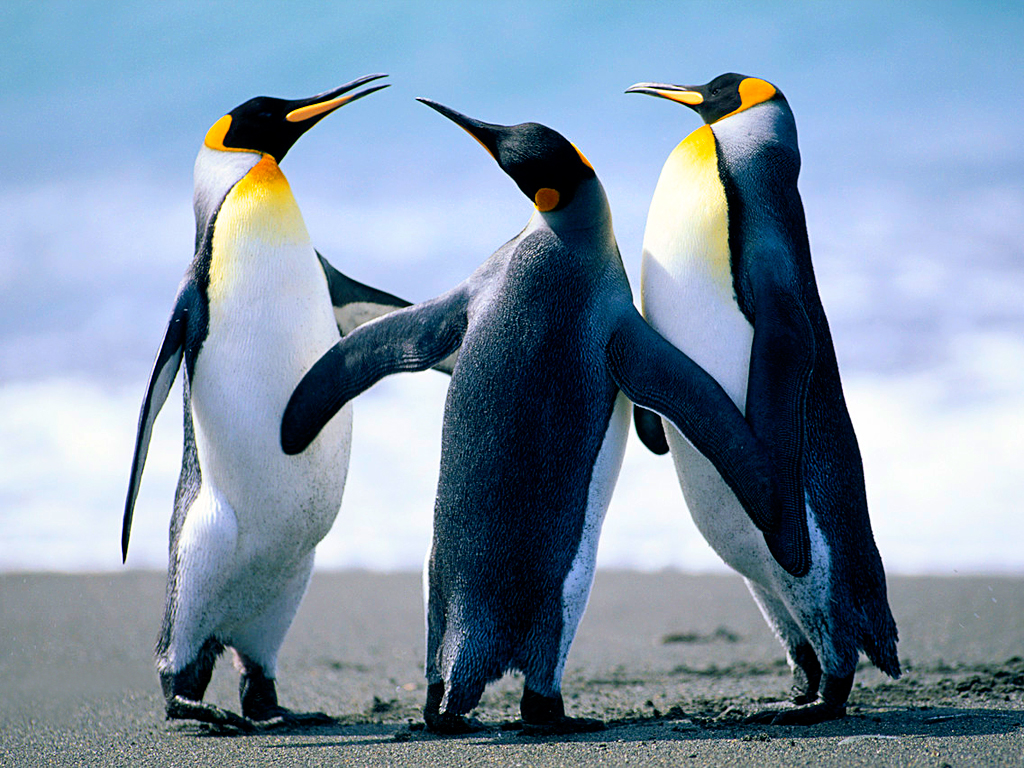
\includegraphics[scale=.50]{figures/Penguins.jpg}
\caption{TAMU figure}
\label{fig:tamu-fig5}
\end{figure}

%%%%%%%%%%%%%%%%%%%%%%%%%%%%%%%%%%%%%%%%%%%%%%%%%%%
%
%  New template code for TAMU Theses and Dissertations starting Fall 2016.
%
%
%  Author: Sean Zachary Roberson 
%	 Version 3.16.09 
%  Last updated 9/12/2016
%
%%%%%%%%%%%%%%%%%%%%%%%%%%%%%%%%%%%%%%%%%%%%%%%%%%%

%%%%%%%%%%%%%%%%%%%%%%%%%%%%%%%%%%%%%%%%%%%%%%%%%%%%%%%%%%%%%%%%%%%%%%
%%                           APPENDIX B
%%%%%%%%%%%%%%%%%%%%%%%%%%%%%%%%%%%%%%%%%%%%%%%%%%%%%%%%%%%%%%%%%%%%%

\chapter{\uppercase {A Second Appendix Whose Title Is Much Longer Than The First}}

Text for the Appendix follows.

\begin{figure}[H]
\centering
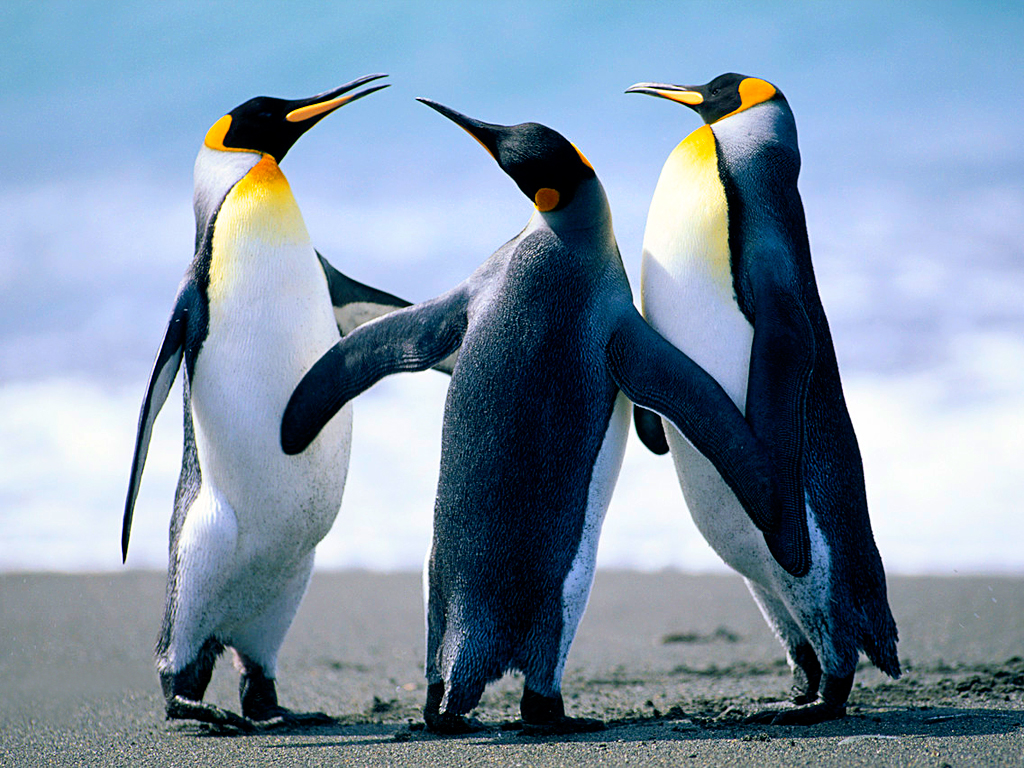
\includegraphics[scale=.50]{figures/Penguins.jpg}
\caption{Another TAMU figure.}
\label{fig:tamu-fig6}
\end{figure}

\section{Appendix Section}

\section{Second Appendix Section}


\pagebreak{}

\end{appendices}


\end{document}
